%%%%%%%%%%%%%%%%%%%%%%%%%%%%%%%%%%%%%%%%%%%%%%%%%%%%%%%%%%%%%%%%%%%%
% bare_jrnl.tex
% V1.4b
% 2015/08/26
% by Michael Shell
% see http://www.michaelshell.org/
% for current contact information.                                                                 
%%%%%%%%%%%%%%%%%%%%%%%%%%%%%%%%%%%%%%%%%%%%%%%%%%%%%%%%%%%%%%%%%%%%

%% This is a skeleton file demonstrating the use of IEEEtran.cls
%% (requires IEEEtran.cls version 1.8b or later) with an IEEE
%% journal paper.
%%
%% Support sites:
%% http://www.michaelshell.org/tex/ieeetran/
%% http://www.ctan.org/pkg/ieeetran
%% and
%% http://www.ieee.org/


\documentclass[journal, onecolumn]{IEEEtran}



%
\usepackage{instructivo}  % Commands for multiple choice
\graphicspath{{./}{./fig/}}

\usepackage[natbib=true,style=trad-unsrt,backend=biber]{biblatex}
\addbibresource{literatura.bib}

\usepackage{standalone}
\usepackage{float}
\usepackage{graphicx}
\usepackage{booktabs}
\usepackage{tabularx}
\usepackage{url}
\usepackage{hyperref}



\renewcommand\IEEEkeywordsname{Palabras clave}
% correct bad hyphenation here
\hyphenation{op-tical net-works semi-conduc-tor}

\begin{document}

\setlength{\parindent}{4.2mm}
%
% paper title
% Titles are generally capitalized except for words such as a, an, and, as,
% at, but, by, for, in, nor, of, on, or, the, to and up, which are usually
% not capitalized unless they are the first or last word of the title.
% Linebreaks \\ can be used within to get better formatting as desired.
% Do not put math or special symbols in the title.
\title{Primer proyecto de aplicación: amplificador de audio}


\author{Matías~A.~Camacho,~\IEEEmembership{Estudiante,~TEC}
        ,~Samantha G.~Cubero,~\IEEEmembership{Estudiante,~TEC}
        ~y~Andrés~Rojas,~\IEEEmembership{Estudiante,~TEC}
}

% The paper headers
\markboth{Taller de diseño analógico, IS2026}%
{Taller de diseño analógico}


% make the title area
\maketitle




\clearpage
\tableofcontents
\clearpage

% Se sugiere no más de cuatro palabras o frases cortas en orden alfabético, separadas por comas, que representen su reporte
\begin{IEEEkeywords}
Diodo, tensión, corriente, junta, ruptura.
\end{IEEEkeywords}


%%%%%%%%%%%%%%%%%%%%%%%%%%%%%%%%%%%%%%%%%%%%%%%%%%%%%%%%%%%%%%%%%%%%%%%%%%%%%%%%%%%%%%%%%%%%%%
%%%%%%%%%%%%%%%%%%%%%%%%%%%%%%%%%%%%%%%%%%%%%%%%%%%%%%%%%%%%%%%%%%%%%%%%%%%%%%%%%%%%%%%%%%%%%%
\section{Introducción}

\subsection{Generación de Formas de Onda}

Es posible producir señales periódicas con características definidas por medio de circuitos analógicos con configuraciones específicas. Entre las señales o formas de onda más comunes se encuentran la onda sinusoidal, la cuadrada y la triangular, las cuales son relevantes para el desarrollo del diseño del presente proyecto. 

Las señales sinusoidales se obtienen típicamente mediante circuitos con osciladores lineales que emplean redes de realimentación selectivas en frecuencia, permitiendo producir señales continuas con baja distorsión, como es el caso del Puente de Wien. Por otro lado, las señales cuadradas se generan a partir de circuitos no lineales que operan en saturación, como comparadores o disparadores tipo Schmitt, produciendo transiciones rápidas entre dos niveles de voltaje \cite{Horowitz1989} .

En el caso de las señales triangulares, estas pueden generarse mediante la integración de una señal cuadrada, tomando en cuenta la relación matemática entre ambas. Un circuito integrador, cuya configuración involucra el uso de amplificadores operacionales, permite transformar una señal de entrada constante en una rampa lineal, dando como resultado una forma de onda triangular cuando la entrada es periódica \cite{Horowitz1989} .

\subsection{Circuitos Comparadores} 

Son circuitos con amplificadores operacionales cuyo funcionamiento se basa en evaluar cuál de sus dos señales de entrada tiene mayor voltaje. Si la señal conectada a la entrada no inversora es mayor que la de la entrada inversora, la salida del comparador cambia a un nivel alto. En caso contrario, cuando la señal en la entrada inversora es mayor, la salida pasa a un nivel bajo. De esta manera, el comparador actúa como un dispositivo que indica, mediante su salida, cuál de las dos entradas predomina en cada instante. A diferencia de los amplificadores operacionales utilizados en configuración lineal, los comparadores operan en modo no lineal o saturación, conmutando rápidamente entre dos niveles de salida. \cite{Mancini2002} . 

\subsection{Modulación por Ancho de Pulso (PWM)}

La modulación por ancho de pulso es una técnica utilizada para representar una señal analógica mediante una señal digital cuyo ciclo de trabajo varía en el tiempo. En este método, la información de la señal de entrada no se transmite mediante cambios en la amplitud, sino a través de la duración relativa de los pulsos en estado alto y bajo dentro de cada período de la señal. El principio de funcionamiento se basa en comparar una señal de referencia, generalmente de baja frecuencia, con una señal portadora de mayor frecuencia, comúnmente de forma triangular o diente de sierra. Cuando la señal de entrada supera a la señal portadora, la salida toma un nivel alto; en caso contrario, la salida permanece en un nivel bajo. Este proceso ocurre de manera continua, generando una señal periódica cuya frecuencia está determinada por la señal portadora. Como resultado, el ciclo de trabajo de la señal PWM varía siguiendo la forma de la señal de entrada: a mayor amplitud de la señal de referencia, mayor es el tiempo que la señal de salida permanece en estado alto dentro de cada período. De esta forma, aunque la señal resultante es digital, conserva la información de la señal analógica original. \cite{hart2011power} .
\subsection{Especificaciones del diseño}


%%%%%%%%%%%%%%%%%%%%%%%%%%%%%%%%%%%%%%%%%%%%%%%%%%%%%%%%%%%%%%%%%%%%%%%%%%%%%%%%%%%%%%%%%%%%%%
%%%%%%%%%%%%%%%%%%%%%%%%%%%%%%%%%%%%%%%%%%%%%%%%%%%%%%%%%%%%%%%%%%%%%%%%%%%%%%%%%%%%%%%%%%%%%%
\section{Diseño}
El proyecto propone diseñar un circuito PWM solo con la utilización de una fuente de DC y varios circuitos con topologías de amplificadores operacionales. Específicamente, se plantea generar una señal sinusoidal con un puente Wien, para compararla (el circuito integrado LM393 funcionando como comparador) con una señal triangular. 

La señal triangular se generará mediante un circuito integrador, el cual será alimentado por una señal cuadrada. Esta señal cuadrada se obtendrá a partir de

Como parámetros de diseño, se tiene que la onda sinusoidal debe tener una frecuencia de 100~Hz y magnitud de 2~V. La onda transportadora debe tener una magnitud de 2.1~V a 2.5~V y una frecuencia de 5~kHz.

Para lograr una frecuencia de 100~Hz con el puente Wien, se utilizó la siguiente fórmula:
\begin{equation}
        f=\frac{1}{2 \pi RC}
\end{equation}

Donde $R$ es la resistencia en el circuito retrasador y $C$ la capacitancia en el circuito retrasador. Esto es suponiendo que todas las resistencias y capacitancias en ese circuito tienen el mismo valor.

Escogiendo una resistencia de 1500~$\Omega$, y una capacitancia de 1~$\mu$F, se obtiene una frecuencia de aproximadamente 106~Hz, lo cual es cercano al valor buscado. Además, los componentes utilizados en la práctica tienen tolerancias que pueden hacer que la frecuencia calculada varíe y esté más cerca o lejos del valor deseado de 100~Hz.


La señal triangular entonces sería generada por un circuito integrador. La frecuencia necesaria es de 5~kHz, la cual está determinada por la señal cuadrada de entrada. La amplitud de la señal triangular dependerá de los valores de los componentes del integrador y de la amplitud de la señal cuadrada.

\section{Simulaciones y análisis}
\subsection{Puentes de Wien}
Para la simulación de los puentes de Wien, se utilizó Multisim. Para poder lograr que los circuitos se iniciaran por sí solos, se utilizó potenciómetros para variar la ganancia y así obtener oscilaciones.
\begin{figure}[H]
        \centering
        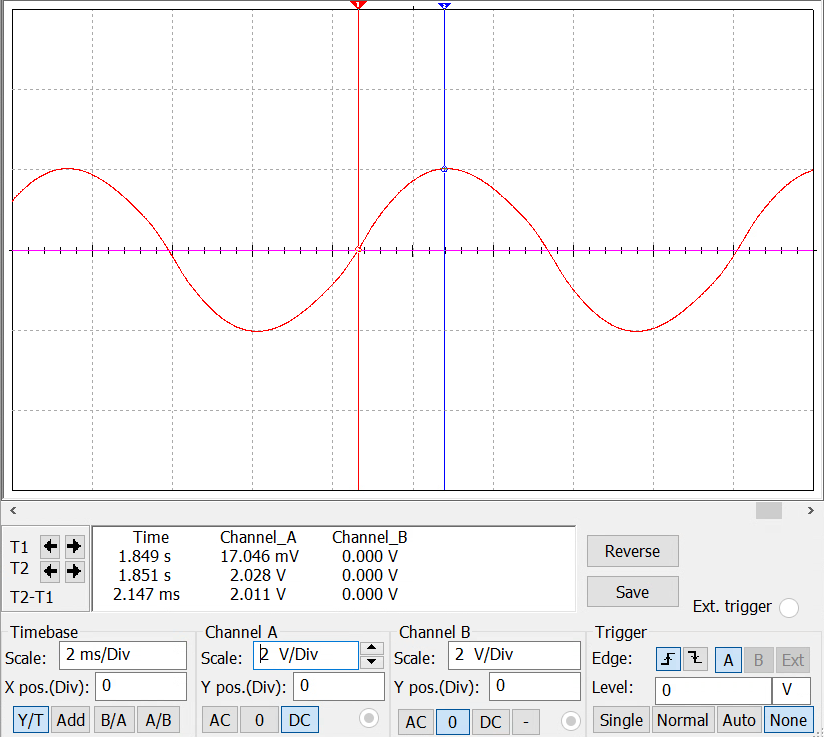
\includegraphics[width=0.6\linewidth]{WienPrimaria.png}
        \caption{Onda de salida del puente de Wien.}
        \label{fig:wienprimaria}
\end{figure}

\section{Resultados Experimentales}





%%%%%%%%%%%%%%%%%%%%%%%%%%%%%%%%%%%%%%%%%%%%%%%%%%%%%%%%%%%%%%%%%%%%%%%%%%%%%%%%%%%%
%%%%%%%%%%%%%%%%%%%%%%%%%%%%%%%%%%%%%%%%%%%%%%%%%%%%%%%%%%%%%%%%%%%%%%%%%%%%%%%%%%%%
\section{Conclusiones}


%%%%%%%%%%%%%%%%%%%%%%%%%%%%%%%%%%%%%%%%%%%%%%%%%%%%%%%%%%%%%%%%%%%%%%%%%%%%%%%%%%%%
%%%%%%%%%%%%%%%%%%%%%%%%%%%%%%%%%%%%%%%%%%%%%%%%%%%%%%%%%%%%%%%%%%%%%%%%%%%%%%%%%%%%
%\appendices





%%%%%%%%%%%%%%%%%%%%%%%%%%%%%%%%%%%%%%%%%%%%%%%%%%%%%%%%%%%%%%%%%%%%%%%%%%%%%%%%%%%%
%%%%%%%%%%%%%%%%%%%%%%%%%%%%%%%%%%%%%%%%%%%%%%%%%%%%%%%%%%%%%%%%%%%%%%%%%%%%%%%%%%%%

\printbibliography

\vfill

\end{document}






